\documentclass[11pt]{article}
\usepackage[letterpaper,margin=1in]{geometry}
\usepackage[T1]{fontenc}
\usepackage{mathptmx}
\usepackage{amsmath,amssymb}
\usepackage{graphicx}
\usepackage{booktabs}
\usepackage[font=small,labelfont=bf]{caption}
\usepackage[numbers,sort&compress]{natbib}
\usepackage{xcolor}
\usepackage{microtype}
\usepackage{authblk}
\usepackage[colorlinks=true,linkcolor=blue!50!black,citecolor=blue!50!black,urlcolor=blue!50!black]{hyperref}
\setlength{\emergencystretch}{3em}
\renewcommand{\baselinestretch}{1.12}
\newcommand{\LIO}{LaInO$_3$}
\newcommand{\BSO}{BaSnO$_3$}
\newcommand{\ns}{n_s}

\title{Intersubband optics of the polar \LIO/\BSO\ two-dimensional electron gas: gate-tunable near-infrared plasmons, phonon-limited lifetimes and intrinsic second-order nonlinearity}
\author{Gracen Ownby}
\affil{University of Oklahoma, Norman, Oklahoma, USA}
\date{\small 12 October 2026}

\begin{document}
\maketitle

\begin{abstract}
The polar interface between \LIO\ and \BSO\ hosts a two-dimensional electron gas (2DEG) whose density can be raised to about $10^{14}$~cm$^{-2}$ by electric-double-layer gating, with low-temperature mobilities above 2000~cm$^2$/Vs. Its optical response has not been studied. We compute the intersubband (ISB) response of this 2DEG from $5\times10^{12}$ to $1.2\times10^{14}$~cm$^{-2}$. The model is a self-consistent Kane-nonparabolic Schr\"odinger--Poisson solution of the interface, with exact in-plane band-edge masses and Fermi-level pinning by compensating acceptors, and a $k$-resolved random-phase (time-dependent Hartree) response that keeps in-plane nonparabolicity, the polar-phonon background and second-order terms. It reduces exactly to the subband-level density-matrix response for a single wavevector shell.

The electrons sit within 0.5--2~nm of the interface, with an in-plane mass of 0.20--0.25~$m_0$, in line with first-principles results. The single-particle transition $E_{21}$ is 0.41--0.59~eV when the bulk \BSO\ is strongly compensated ($N_A=5\times10^{19}$~cm$^{-3}$) and 0.13--0.44~eV when it is not ($10^{18}$~cm$^{-3}$). The depolarization shift is large because the background permittivity at these energies is only about 4: the centroid of the collective absorption moves from 0.53 to 0.93~eV and from 0.28 to 0.81~eV over the density range, 1.3--2.4 times $E_{21}$, so that the gate tunes the absorption across 1.3--4.4~$\mu$m. The plasmon hybridizes with the higher $1\to n$ transitions, and at $10^{14}$~cm$^{-2}$ no single mode carries more than 28\% of the absorption. The polar phonons shift the centroid by at most 8~meV; local exchange and correlation raise it by 1--8\%, depending on how they are screened.

For a 1.6~eV conduction-band offset and a field-free cap, the Fermi level reaches the \LIO\ conduction band near $1.25\times10^{14}$~cm$^{-2}$ in the compensated case, and at lower density if part of the gate charge sits on the cap surface; this limits useful gating. With three polar LO modes (Fr\"ohlich constants summing to 1.3) the $2\to1$ lifetime of the electrons created by ISB absorption is 32--79~fs, including Pauli blocking and static screening, which is weak because the intersubband transition density couples only weakly to the 2DEG. The asymmetric well has an intrinsic second-order susceptibility. Coulomb screening reduces it by factors of 2--9, and for a 30~meV linewidth the sheet value of one interface is 37--137~nm$^2$/V, 0.07--0.25 of one period of a doubly resonant InGaAs/InAlAs asymmetric double well, with a resonance that the gate tunes across the mid-infrared. UQABSTRACT
\end{abstract}

\section{Introduction}
\BSO\ is a wide-gap perovskite (indirect gap about 3.0~eV) with a dispersive Sn-5s conduction band and a band-edge mass of about 0.19~$m_0$ \cite{Niedermeier2017,Aggoune2022}. When \LIO\ is grown on it, the polar discontinuity between the neutral BaO/SnO$_2$ planes and the charged LaO$^+$/InO$_2^-$ planes creates a 2DEG on the \BSO\ side of the interface without intentional doping \cite{Kim2019LIO,Aggoune2021}. Electric-double-layer gating has raised its density to about $10^{14}$~cm$^{-2}$, with mobilities above 2000~cm$^2$/Vs at 10~K \cite{Lee2024LIO}. The conduction-band offset is about 1.6~eV \cite{Kim2019LIO,Lee2024LIO}, and first-principles calculations place the 2DEG within 1--2~nm of the interface with a mass of 0.24~$m_0$ \cite{Aggoune2021}. All of this work concerns transport.

A strongly confined, dense 2DEG with a light mass and a large band offset is also an intersubband (ISB) system, and an unusual one. Its background permittivity at near-infrared frequencies is about 4, against 10--13 in III--V wells, so Coulomb effects on the ISB response are large. It is polar, so its ISB transitions couple strongly to LO phonons. And its confining potential is asymmetric by construction, so it has a second-order nonlinearity without compositional engineering. Oxide ISB optics is a young field: room-temperature ISB absorption has been measured in SrTiO$_3$/LaAlO$_3$ wells \cite{Ortmann2018}, and \BSO\ quantum wells with BaO, MgO or Al$_2$O$_3$ barriers have been modelled \cite{Li2021BSO,Stanojevic2023,Jang2023}. Those studies use La-doped wells, parabolic bands, a fixed linewidth and no depolarization or phonons; the largest second-order susceptibilities predicted are 200~nm/V under bias \cite{Li2021BSO}. A comparable treatment exists for $\beta$-Ga$_2$O$_3$ wells \cite{Lyman2020}. The polar \LIO/\BSO\ 2DEG has not been treated.

This paper computes its ISB response as a function of the gated density. The results are: (i) the subband structure, including how strongly the compensating acceptors in the \BSO\ set the confinement, and the density at which the Fermi level reaches the \LIO\ conduction band (Sec.~\ref{sec:sub}); (ii) the collective ISB response with in-plane nonparabolicity, which lies 30--140\% above $E_{21}$, splits among hybrid modes and tunes from the mid- to the near-infrared (Sec.~\ref{sec:lin}); (iii) LO-phonon lifetimes with all three polar modes, Pauli blocking and screening (Sec.~\ref{sec:tau}); (iv) the intrinsic second-order susceptibility (Sec.~\ref{sec:chi2}); and (v) a Monte Carlo propagation of the uncertainty in the material parameters (Sec.~\ref{sec:uq}). The calculations use qwkit \cite{qwkit}, extended for this work with a single-interface solver and a $k$-resolved collective response.

\section{Model}\label{sec:model}
\subsection{Material parameters}
Table~\ref{tab:par} lists the parameters and their ranges, from the sources compiled for this work. The \BSO\ band-edge mass and Kane nonparabolicity come from infrared measurements over $1.6\times10^{19}$--$7.3\times10^{20}$~cm$^{-3}$, which give $m^*=0.19\,m_0$ and $\beta=0.56$~eV$^{-1}$ in $E(1+\beta E)=\hslash^2k^2/2m^*$ \cite{Niedermeier2017}; first-principles calculations give 0.20~$m_0$ and $\beta=0.25$~eV$^{-1}$ \cite{Krishnaswamy2017}. The three polar modes of \BSO\ are taken from infrared ellipsometry \cite{Stanislavchuk2012}. With $\varepsilon_\infty=4.0$, the value at the ISB energies of interest, their factorized dielectric function gives $\varepsilon_0=20.5$, consistent with the static values in use (17--20). The \LIO\ phonons are not known, so the cap is treated as a passive barrier. Kim \emph{et al.} found deep acceptors of $4$--$6\times10^{19}$~cm$^{-3}$ in their \BSO\ films \cite{Kim2019LIO}; we use $5\times10^{19}$~cm$^{-3}$ as the strongly compensated case and $10^{18}$~cm$^{-3}$ as a cleaner film, and pin the Fermi level 1.0~eV below the bulk conduction band (0.5--1.5~eV in Sec.~\ref{sec:uq}).

\begin{table}[t]
\centering\small
\caption{Parameters (baseline and range used in Sec.~\ref{sec:uq}).}\label{tab:par}
\begin{tabular}{lll}
\toprule
Quantity & Baseline & Range, source \\
\midrule
\BSO\ band-edge mass $m^*$ & 0.19~$m_0$ & 0.17--0.22 \cite{Niedermeier2017,Krishnaswamy2017,Aggoune2022} \\
\BSO\ nonparabolicity $\beta$ & 0.56~eV$^{-1}$ & 0.25--0.56 \cite{Niedermeier2017,Krishnaswamy2017} \\
\BSO\ $\varepsilon_s$ (Poisson) & 20 & $\varepsilon_\infty\prod_j(\omega_{Lj}/\omega_{Tj})^2$: 16.9--22.0 \cite{Stanislavchuk2012,Krishnaswamy2017} \\
\BSO\ $\varepsilon_\infty$ (ISB energies) & 4.0 & 3.3--4.3 \cite{Stanislavchuk2012,Krishnaswamy2017,Aggoune2022} \\
\BSO\ TO/LO (cm$^{-1}$) & 135/154, 244.5/421, 628/723 & \cite{Stanislavchuk2012} \\
\LIO/\BSO\ conduction-band offset & 1.6~eV & 1.35--1.70 \cite{Kim2019LIO,Lee2024LIO,Aggoune2021} \\
\LIO\ mass, $\varepsilon_s$ & 0.46~$m_0$, 24 & 0.30--0.50 \cite{Kim2019LIO,Aggoune2021,Jang2017LIO} \\
Acceptors in \BSO\ $N_A$ & $5\times10^{19}$, $10^{18}$~cm$^{-3}$ & $10^{18}$--$5\times10^{19}$ (log) \cite{Kim2019LIO} \\
Pinning $E_c-E_F$ in bulk \BSO & 1.0~eV & 0.5--1.5 (assumed) \\
ISB linewidth (HWHM) & 10~meV & 30~meV as an alternative (Sec.~\ref{sec:tau}) \\
\bottomrule
\end{tabular}
\end{table}

\subsection{Self-consistent interface}
The \LIO\ cap ($-d<z<0$, $d=5$~nm, closed by a hard wall that stands for the electrolyte) and the \BSO\ ($0<z<L$) are described by a one-band Kane Schr\"odinger equation with an energy-dependent mass $m(z,E)=m^*(z)[1+(E-V(z))\beta(z)]$ \cite{Nelson1987}, $H(E,k)=-\partial_z\frac{\hslash^2}{2m(z,E)}\partial_z+V(z)+\frac{\hslash^2k^2}{2m(z,E)}$. The in-plane band-edge mass of subband $n$ follows from first-order perturbation theory in $k^2$ with the energy dependence of $H$ \cite{Ekenberg1989},
\begin{equation}
\frac{1}{m_n}=\frac{\langle m(z,E_n)^{-1}\rangle_n}{1-\langle\partial_EH\rangle_n},\qquad \langle\partial_EH\rangle_n=-\frac{\hslash^2}{2}\int\frac{m^*\beta}{m(z,E_n)^2}\,|\psi_n'|^2\,dz,\label{eq:mass}
\end{equation}
which reduces to the bulk Kane result $m^*(1+2\beta T)$ for a flat well with kinetic energy $T$. The in-plane dispersion is written as
\begin{equation}
\frac{\hslash^2k^2}{2m_n}=\epsilon\left(1+\frac{\epsilon}{G_n}\right),\label{eq:disp}
\end{equation}
with $G_n$ fitted to the exact dispersion $E_n(k)$ of $H(E,k)$ over the occupied range (it reproduces $E_n(k)$ to 0.5\%); the subband density of states is then $(m_n/\pi\hslash^2)(1+2\epsilon/G_n)$, with Fermi--Dirac occupations. The Hartree potential is generated by the electrons, by ionized acceptors over a depletion width $w_d$, and by a positive sheet (polarization and gate charge) that neutralizes them. The depletion width follows from Fermi-level pinning in the bulk \BSO, $V(L)-E_F=E_\mathrm{pin}$. In the baseline the positive sheet sits at the interface, so that the cap is field-free; Sec.~\ref{sec:sub} shows what happens when part of it sits on the cap surface. A local exchange-correlation potential (Hedin--Lundqvist \cite{HedinLundqvist1971}) is used as a check. The equations are solved with Anderson mixing, first with an approximate nonparabolicity and then with the fitted $G_n$ held fixed; the box length is $L=1.4\,w_d^{0}+15$~nm, clipped to 30--250~nm, where $w_d^0$ is the depletion width of the pinning voltage alone.

\subsection{$k$-resolved collective response}
The subband wavefunctions at $k=0$ are kept, and each in-plane wavevector shell carries the occupations $f_n(k)$ and energies $E_n(k)$ of Eq.~\eqref{eq:disp}. The shells are coupled only through the Hartree potential of the total induced density. For a $z$-polarized drive, given as the field $E_d=D/\varepsilon_b$ the stack would have without the electrons,
\begin{align}
(\hslash\omega-E_{ab}(k)+i\gamma)\,\rho^{(1)}_{ab}(k)&=[f_b(k)-f_a(k)]\,\tilde U_{ab},\qquad \tilde U=eE_dz+U_H[X^{(1)}],\quad X^{(1)}=\sum_k w_k\rho^{(1)}(k),\\
U_H[X]_{ab}&=\frac{e^2}{\varepsilon_0\varepsilon_b(\omega)}\sum_{cd}S_{abcd}X_{cd},\qquad S_{abcd}=\int F_{ab}F_{cd}\,dz,\quad F_{ab}(z)=\int_{-\infty}^z\psi_a\psi_b\,dz',
\end{align}
where $w_k$ is the sheet density of a shell ($k\,dk/\pi$, spin included) and $E_{ab}=E_a-E_b$. The induced sheet dipole is $p=-e\sum_{ab}z_{ba}X_{ab}$, and the absorbed power per unit area is $(\omega/2)\,\mathrm{Im}\,p\,|E_d|^2$; for a thin layer this is the loss function measured in Brewster-angle or attenuated-total-reflection geometries. At second order,
\begin{align}
(2\hslash\omega-E_{ab}(k)+i\gamma)\,\rho^{(2)}_{ab}(k)&=[\tilde U,\rho^{(1)}(k)]_{ab}+[f_b(k)-f_a(k)]\,U_H[X^{(2)}]_{ab}\quad(a\neq b),\\
(2\hslash\omega+i\hslash/\tau_p)\,\rho^{(2)}_{aa}(k)&=[\tilde U,\rho^{(1)}(k)]_{aa},
\end{align}
with $U_H$ evaluated with $\varepsilon_b(2\omega)$, $X^{(2)}=\sum_kw_k\rho^{(2)}(k)$ and $\chi^{(2)}_s=-e\sum_{ab}z_{ba}X^{(2)}_{ab}/\varepsilon_0E_d^2$. The population time $\tau_p=1$~ps only enters the diagonal terms at $2\omega$, where it is irrelevant ($2\hslash\omega\gg\hslash/\tau_p$). The background permittivity $\varepsilon_b(\omega)=\varepsilon_\infty\prod_j(\omega_{Lj}^2-\omega^2-i\omega g)/(\omega_{Tj}^2-\omega^2-i\omega g)$ contains the three polar modes ($\hslash g=2$~meV). With a single shell and no dispersion the equations reduce exactly to the subband-level time-dependent Hartree response \cite{AllenTsuiVinter1976,Ando1977,AndoRMP1982} already in qwkit (agreement to $10^{-8}$ in the test suite); with the Hartree term off they give the single-particle response. Pairs of subbands that are both empty carry no first-order coherence and are dropped from the linear system (occupation differences below $10^{-5}$). All subbands up to 3~eV above $E_1$ (at most 90, which reach 2.1--2.6~eV in the cleaner case) and 200 shells are used; Sec.~\ref{sec:lin} gives the convergence. Because the subbands are eigenstates of different energy-dependent Hamiltonians, their envelopes overlap slightly; they are L\"owdin-orthonormalized as a set that extends 0.6~eV beyond the kept range, so that the truncation does not distort the highest kept states. In the two-band Kane model from which the energy-dependent mass derives, the states including their valence components are orthogonal without this step (to $2\times10^{-3}$ on our grids), and the two-band dipoles agree with the L\"owdin ones: $z_{12}$ to 0.6\%, the $1\to n$ oscillator-strength sum to 1.5\% and its centroid to 1.2\%. When the two-band transition densities are also used in the Hartree kernel, the collective centroids are 2.2--2.6\% lower and the single-particle ones 0.5--0.7\% lower than in the baseline.

\subsection{LO phonons}
Each polar mode $j$ couples with the Fr\"ohlich factor $C_j=(1/\varepsilon_\infty-1/\varepsilon_0)_j$ obtained from the residue of $1/\varepsilon_b(\omega)$ at its LO pole; the $C_j$ sum to $1/\varepsilon_\infty-1/\varepsilon_0$ \cite{Varga1965}. The corresponding Fr\"ohlich constants for $m^*=0.19\,m_0$ are 0.12, 0.76 and 0.45 for the 19, 52 and 90~meV modes. The rate out of an electron of wavevector $k$ in subband 2 into subband 1 is the bulk-phonon rate \cite{Ridley1982} generalized to $k\neq0$: an angular integral over the final wavevector of $I_{21}(Q)/Q$, with $I_{21}$ the Coulomb form factor and $Q=|\mathbf k-\mathbf k'|$, the nonparabolic final density of states of Eq.~\eqref{eq:disp}, the phonon occupation, and Pauli blocking $1-f_1(k')$. It is averaged over the electrons that an intersubband absorption creates, vertical transitions from subband 1 with weight $f_1(k)[1-f_2(k)]$. Screening by the 2DEG is static RPA screening of the $2\to1$ vertex by the intrasubband polarization of the occupied subbands, with the two-dimensional Lindhard function and the Coulomb form factors $F_{21,ll}(Q)$ and $F_{ll,mm}(Q)$ (background $\varepsilon_\infty$). It is weak, because the intersubband transition density $\psi_1\psi_2$ couples only weakly to the monopole density of the 2DEG.

\section{Subband structure and the gating limit}\label{sec:sub}
Figure~\ref{fig:sub}a shows the self-consistent potential at $3\times10^{13}$ and $10^{14}$~cm$^{-2}$ for the strongly compensated case. The well is triangular near the interface. The depletion charge of the acceptors, $4.1\times10^{13}$~cm$^{-2}$ over 8~nm, is comparable to the 2DEG and steepens the well. The mean distance of the ground subband from the interface falls from 8.1 to 4.9~\AA\ as the density rises from $5\times10^{12}$ to $1.2\times10^{14}$~cm$^{-2}$; with $10^{18}$~cm$^{-3}$ acceptors (depletion charge $5\times10^{12}$~cm$^{-2}$ over 51~nm) it falls from 18 to 6.2~\AA. The in-plane band-edge mass of the ground subband, Eq.~\eqref{eq:mass}, is 0.23--0.25~$m_0$ and 0.20--0.24~$m_0$ in the two cases, close to the 0.24~$m_0$ of first-principles calculations \cite{Aggoune2021}, and the 2DEG lies within the 1--2~nm found there. A mean distance of 5--8~\AA\ is 1.2--2 \BSO\ unit cells. The envelope-function approximation is then at its limit: Li \emph{et al.} found effective-mass and Wannier tight-binding levels in agreement for \BSO\ wells of 3--7 unit cells \cite{Li2021BSO}, which does not cover the densest cases here. The predictions at the highest densities are therefore indicative.

\begin{figure}[t]
\centering
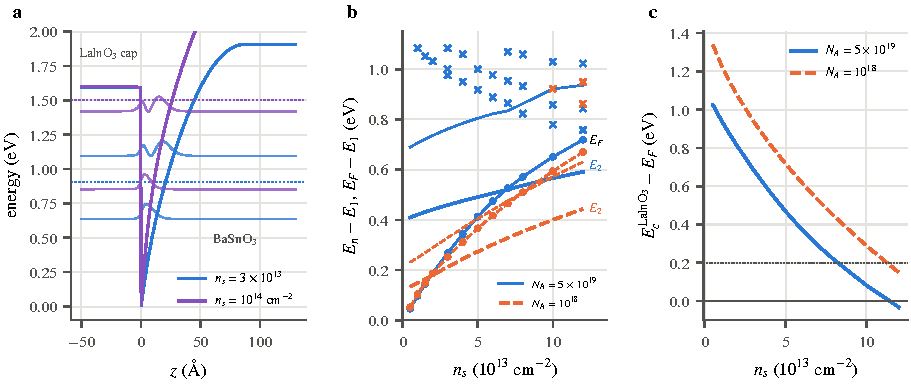
\includegraphics[width=\textwidth]{figures/fig1_subbands.pdf}
\caption{(a) Self-consistent conduction band, first two subbands (offset by their energies) and Fermi level (dotted) at $\ns=3\times10^{13}$ and $10^{14}$~cm$^{-2}$, $N_A=5\times10^{19}$~cm$^{-3}$, 300~K; energies from the conduction band at the interface. (b) $E_2-E_1$ (thick), $E_3-E_1$ (thin) and $E_F-E_1$ (dots) against density for the two acceptor densities. (c) Distance of the Fermi level below the \LIO\ conduction band (field-free cap).}
\label{fig:sub}
\end{figure}

The single-particle transition energy $E_{21}$ is 0.41--0.59~eV for $N_A=5\times10^{19}$~cm$^{-3}$ and 0.13--0.44~eV for $10^{18}$~cm$^{-3}$ over $5\times10^{12}$--$1.2\times10^{14}$~cm$^{-2}$ (Fig.~\ref{fig:sub}b): the compensation of the bulk \BSO\ shifts it by up to 0.28~eV at equal density. The second subband starts to fill at $6\times10^{13}$~cm$^{-2}$ in the compensated case and already below $10^{13}$~cm$^{-2}$ in the clean case, where it holds about a fifth of the electrons from $5\times10^{13}$~cm$^{-2}$ on.

The Fermi level rises by 0.67~eV above $E_1$, and by 1.2--1.6~eV above the conduction band at the interface, over the density range. With a field-free cap it comes within 0.2~eV of the \LIO\ conduction band at $9\times10^{13}$~cm$^{-2}$ and reaches it at about $1.25\times10^{14}$~cm$^{-2}$ in the compensated case (Fig.~\ref{fig:sub}c); for cleaner \BSO\ the margin is still 0.22~eV at $1.2\times10^{14}$~cm$^{-2}$. Beyond that point the states of the 5~nm cap fill and conduction becomes parallel. The field-free cap is the favourable limit. If part of the positive sheet sits on the cap surface instead of at the interface, as when the gate charge is not fully transferred, the cap carries a field that lowers its conduction band at the interface: with 10\% of the sheet on the surface the margin at $10^{14}$~cm$^{-2}$ is already negative ($-0.23$ and $-0.11$~eV in the two cases), and with 25\% the Fermi level reaches the cap conduction band already at $3\times10^{13}$~cm$^{-2}$ in the compensated case. How the polarization and gate charges are distributed in an electrolyte-gated stack is not known. This limit lies close to the highest gated densities reported, about $10^{14}$~cm$^{-2}$ \cite{Lee2024LIO,Ueno2008}.

\section{Collective intersubband response}\label{sec:lin}
Figure~\ref{fig:spec} maps the absorbed power against photon energy and density. The single-particle spectra (a, b) follow $E_{21}$, slightly red-shifted by in-plane nonparabolicity: the upper subband is heavier, so the $1\to2$ energy falls with $k$. Across the Fermi sea the $1\to2$ energy falls by about $(1-m_1/m_2)(E_F-E_1)$. In the compensated case the masses differ by 8--10\%, and the single-particle $1\to2$ line (full width on the 5~meV grid) widens from 15~meV at low density to 35~meV at $8\times10^{13}$~cm$^{-2}$ and 55--80~meV at 1--$1.2\times10^{14}$~cm$^{-2}$, against 20~meV from the assumed homogeneous width. In the clean case the masses differ by less than 3\% and the line stays at 15--20~meV. In the compensated case the $1\to3$ and higher transitions are weak ($z_{13}\le1.25$~\AA\ against $z_{12}=4.3$--5.4~\AA). In the clean case the dense ladder of states on the shallow depletion slope gives several transitions of comparable strength.

\begin{figure}[t]
\centering
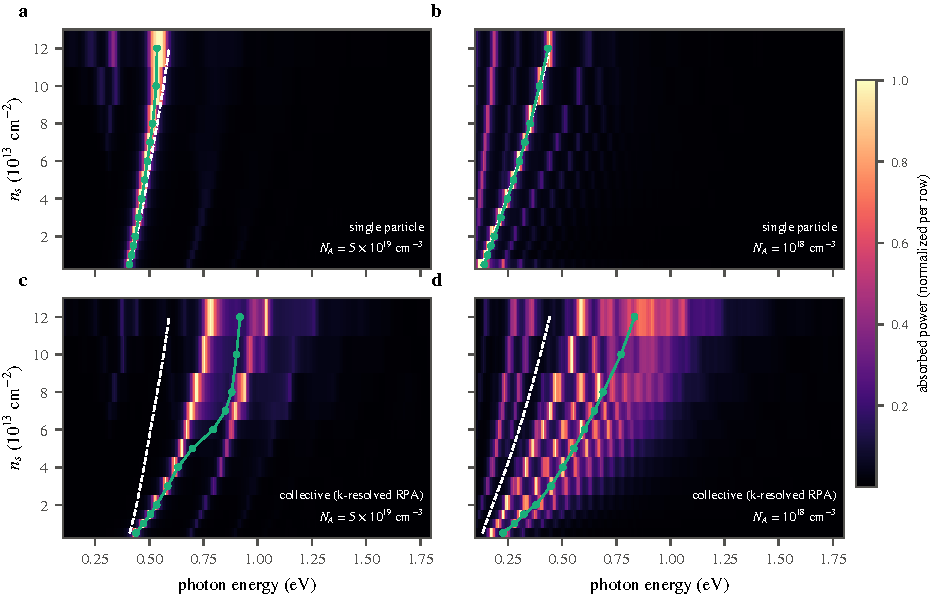
\includegraphics[width=\textwidth]{figures/fig2_spectra.pdf}
\caption{Absorbed power against photon energy (each row normalized to its maximum) for single-particle (a, b) and collective (c, d) response, $N_A=5\times10^{19}$ (a, c) and $10^{18}$~cm$^{-3}$ (b, d), 300~K, $\gamma=10$~meV. White dashed lines: $E_{21}$. Green dots: centroid of the absorption over 0.10--2.5~eV.}
\label{fig:spec}
\end{figure}

The collective response (c, d) is shifted far to the blue. Its centroid rises from 0.53 to 0.93~eV in the compensated case and from 0.28 to 0.81~eV in the clean case (Fig.~\ref{fig:coll}a). Relative to the single-particle centroid it is 1.07--1.70 (compensated) and 1.25--1.82 (clean) times higher, the ratio growing with density in both cases; relative to $E_{21}$ it is 1.3--1.7 and 1.9--2.4 times higher. The shift is large because the density is about 100 times that of a typical III--V ISB structure while the background permittivity at these energies, about 4, is a third of the III--V value \cite{AllenTsuiVinter1976,Ando1977}. The gate tunes the collective absorption across 1.3--4.4~$\mu$m.

\begin{figure}[t]
\centering
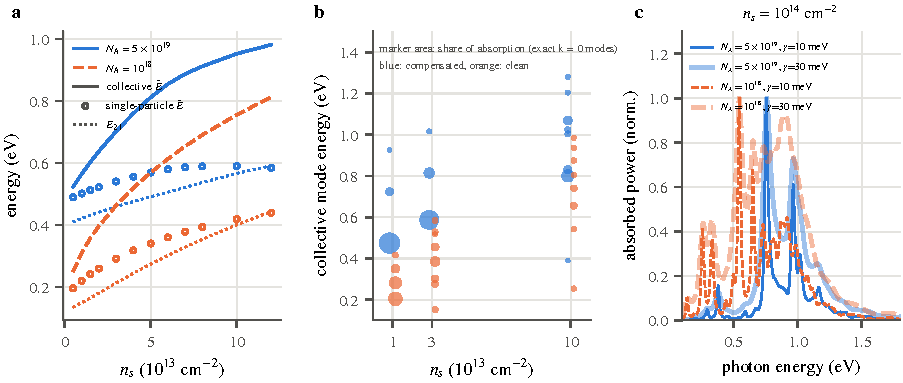
\includegraphics[width=\textwidth]{figures/fig3_collective.pdf}
\caption{(a) Centroid of the collective (solid, dashed) and single-particle (open symbols) absorption, and $E_{21}$ (dotted). (b) Collective modes of the $k=0$ response with $\gamma=2$~meV at three densities; marker area is the share of the absorption carried by each mode (blue, $N_A=5\times10^{19}$; orange, $10^{18}$~cm$^{-3}$). (c) Collective spectra at $10^{14}$~cm$^{-2}$ for $\gamma=10$ and 30~meV.}
\label{fig:coll}
\end{figure}

The collective oscillator strength does not stay in one mode. In the heavily doped III--V wells of Refs.~\cite{Delteil2012,Vasanelli2020}, Coulomb coupling concentrates the strength of many transitions into one narrow multisubband plasmon. Here the depolarization shift of the $1\to2$ transition becomes comparable to the spacing of the $1\to3$, $1\to4$ and (once it fills) $2\to n$ transitions, and the modes hybridize. The mode analysis of Fig.~\ref{fig:coll}b makes this explicit. In the compensated case one mode carries 79\% of the absorption at $10^{13}$~cm$^{-2}$ and 67\% at $3\times10^{13}$~cm$^{-2}$, but at $10^{14}$~cm$^{-2}$ the largest share is 28\%, with four modes between 0.80 and 1.06~eV carrying two-thirds of the total. In the clean case the strength is already shared among several modes at $10^{13}$~cm$^{-2}$ (31\%, 29\% and 14\% for the three largest). Correspondingly, the fraction of the absorption within 50~meV of the strongest peak falls from 0.72 to 0.28 (compensated) and from 0.47 to 0.14 (clean) as the density rises, while for the single-particle spectra it stays at 0.37--0.74. The splitting survives a broader line: with $\gamma=30$~meV the fraction is 0.22--0.53 and 0.12--0.40 (Fig.~\ref{fig:coll}c). The centroids then move up by 2--6\%, and by up to 18\% at the lowest densities of the clean case, because the broader Lorentzian tails are weighted by $\omega$ in the absorbed power and cut at 0.1~eV.

The $k=0$ response (all electrons at the subband edges, used for the mode analysis) gives centroids 1--5\% above the $k$-resolved ones and strongest peaks up to 50~meV higher: in-plane nonparabolicity is a minor effect here because the subbands have similar masses, and the $k$-resolution mainly red-shifts the modes slightly and sets their line shapes. The numerical parameters are converged. With 400 instead of 200 shells the spectra are unchanged to $10^{-4}$; halving the grid step (to 0.25~\AA\ in the compensated and 0.5~\AA\ in the clean case) raises $E_{21}$ by 1--3~meV and the collective centroids by at most 0.9\%. Subbands up to 2 instead of 3~eV above $E_1$ change the centroids by at most 0.6\%, and up to 4~eV by less than 0.1\%; in the clean case, where the 90 subbands reach 2.1--2.6~eV, extending the single-particle $1\to n$ sum to 3~eV moves its centroid by 0.3\%. Doubling the box changes $E_{21}$ by at most 1~meV and the centroids by at most 0.4\%. In a few runs the residual of the self-consistent potential stalls at 2--10~meV (an oscillation of the depletion edge); at $5\times10^{12}$~cm$^{-2}$ (compensated), the worst case, $E_{21}$ and $E_F$ change by less than 0.1~meV between runs with different mixing. The response satisfies the $f$-sum rule: with a constant background $\varepsilon_\infty$, the absorption integrated over 0.02--4~eV is the same for the single-particle and collective spectra to $10^{-4}$ (at $10^{14}$~cm$^{-2}$, compensated, and $10^{13}$~cm$^{-2}$, clean); the Coulomb coupling redistributes the oscillator strength without creating it. Local exchange and correlation in the self-consistent potential (Hedin--Lundqvist, screened by $\varepsilon_s$) raise $E_{21}$ by 6--10~meV and the collective centroids by 1--2.4\%. Screened by $\varepsilon_\infty$ instead, an upper limit for their strength at these energies, they raise $E_{21}$ by 38--59~meV and the centroids by 5--11\%; the corresponding adiabatic local kernel in the response (time-dependent local-density approximation) takes back part of this, leaving 1--8\%. Without the polar phonons in the background (constant $\varepsilon_\infty$) the centroids are 0.1--1.7\% (at most 8~meV) lower, and a 3~nm instead of a 5~nm cap changes them by less than 1\%. At 10~K the centroids differ from the 300~K values by at most 1.2\%, because the 2DEG is degenerate.

\section{LO-phonon lifetimes}\label{sec:tau}
\BSO\ couples strongly to its polar phonons: the Fr\"ohlich constants sum to 1.3. The 52 and 90~meV modes contribute about equally to the $2\to1$ rate (43--45\% and 51--54\%), the 19~meV mode 3\%. Figure~\ref{fig:life}a shows the lifetime of the electrons that an intersubband absorption places in subband 2, with Pauli blocking and static screening, and two simpler estimates. In the compensated case it is 34--53~fs, rising with density because $E_{21}$ moves away from the LO energies and the emission wavevector grows. In the clean case it is 32--79~fs. This corresponds to a lifetime contribution $\hslash/2\tau$ of 4--10~meV to the half-width, comparable to the assumed 10~meV.

The corrections to the edge rate are moderate. Averaging over the excited electrons shortens the lifetime by about 17\% in the compensated case, because electrons at finite $k$ can emit at smaller wavevector transfer; in the clean case, where $E_{21}$ is close to the LO energies, it changes it by $-4$ to $+12$\%. Pauli blocking of the final states in subband 1 matters once $E_F-E_1$ exceeds the LO energies: it lengthens the lifetime by up to 14\% (compensated) and 60\% (clean). Screening is weak. The intersubband transition density $\psi_1\psi_2$ couples to the intrasubband polarization of the 2DEG only through the overlap of the form factors, so the static RPA factor at the emission wavevector is 0.89--0.97 (compensated) and 0.72--0.90 (clean), and screening lengthens the lifetime by 3--12\% and 14--34\%. Static screening needs $\hslash Qv_F$ well above the LO energy. The factor is 2.7--22 in the compensated case, but only 1.1--2.5 in the clean case at the lowest densities, and the dynamic screening, which is weaker, would leave the lifetime nearer the unscreened value. Treating the 2DEG as a two-dimensional Thomas--Fermi screen of the bare Fr\"ohlich vertex would overstate the screening badly, because it ignores the form factors.

For comparison, the transport mobility of 2100~cm$^2$/Vs at 10~K corresponds to $\hslash/\tau_\mathrm{tr}\approx2.8$~meV, and 80~cm$^2$/Vs at room temperature to about 70~meV \cite{Lee2024LIO,Ngabonziza2024}. At room temperature the transport rate is dominated by intrasubband LO scattering, which does not broaden the intersubband line in the same way; ISB linewidths are usually broader than the transport value at low temperature because interface roughness acts on the intersubband transition directly. A linewidth of 10--30~meV, the range used here, is therefore a reasonable expectation.

\begin{figure}[t]
\centering
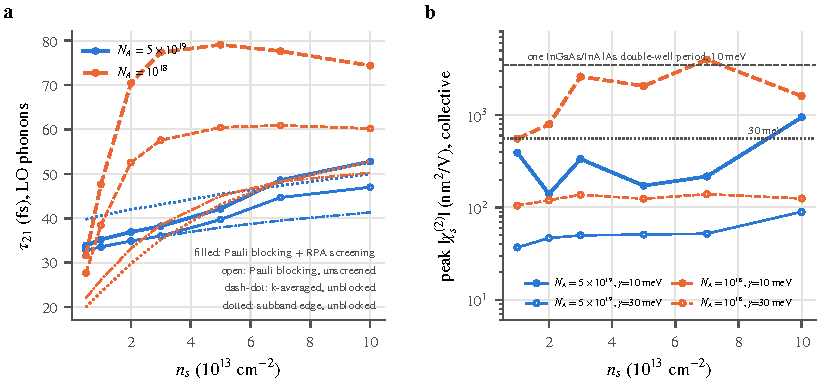
\includegraphics[width=\textwidth]{figures/fig4_lifetime_chi2.pdf}
\caption{(a) LO-phonon $2\to1$ lifetime of the electrons created by intersubband absorption, with Pauli blocking and static RPA screening (filled), with Pauli blocking only (open), and for an electron at the bottom of subband 2 without either (dotted), 300~K. (b) Peak sheet second-order susceptibility of the collective response over pump energies of 0.10--1.2~eV for $\gamma=10$~meV (filled) and 30~meV (open). Grey lines: one 21.4~nm period of a doubly resonant InGaAs/InAlAs asymmetric double well at $5\times10^{11}$~cm$^{-2}$, computed with the same collective code, for $\gamma=10$ (dashed) and 30~meV (dotted).}
\label{fig:life}
\end{figure}

\section{Second-order nonlinearity}\label{sec:chi2}
The triangular polar well breaks inversion symmetry, so $\chi^{(2)}_{zzz}$ is nonzero without compositional asymmetry, and its magnitude follows the gate. For a single interface we report the sheet susceptibility for second-harmonic generation, $\chi^{(2)}_s=P^{(2)}_\mathrm{sheet}/\varepsilon_0E_d^2$, and take the peak of its modulus over pump energies of 0.10--1.2~eV (0.01~eV grid, refined to 1~meV around the three largest maxima). We give it for $\gamma=10$ and 30~meV; the second is the realistic width at room temperature (Sec.~\ref{sec:tau}).

In the single-particle response of the compensated case the peak lies at $2\hslash\omega\approx E_{21}$ up to $7\times10^{13}$~cm$^{-2}$, where the two-level term $z_{12}^2(z_{22}-z_{11})$ of the asymmetric well dominates; in the clean case, with its denser ladder of states, several resonances compete and the peak lies at pump energies of 0.10--0.14~eV. The peak is 180--550~nm$^2$/V ($\gamma=10$~meV) and 65--210~nm$^2$/V (30~meV) in the compensated case, and 2100--5200 and 660--1090~nm$^2$/V in the clean case, where the less confined states have longer dipoles ($z_{12}=9.0$ against 5.3~\AA\ at $10^{13}$~cm$^{-2}$). At the two lowest densities of the clean case the 30~meV peak lies at the lower end of the pump range, next to the 90~meV LO phonon, and is a lower bound.

The Coulomb coupling changes this picture. The depolarization field screens the drive below the collective resonances, at $\omega$ and at $2\omega$, and moves the resonances to the hybrid-mode energies of Sec.~\ref{sec:lin}. With $\gamma=30$~meV the collective peak is 37--90~nm$^2$/V in the compensated case and 105--137~nm$^2$/V in the clean case (Fig.~\ref{fig:life}b), 1.8--4.1 and 5.5--9.0 times below the single-particle values, at pump energies of 0.24--0.38 and 0.12--0.23~eV. With $\gamma=10$~meV the collective peaks, 140--940 and 540--3700~nm$^2$/V, vary irregularly with density. They occur where one hybrid mode lies at $\hslash\omega$ and another at $2\hslash\omega$: at $10^{13}$~cm$^{-2}$ in the compensated case, for example, the pump at 0.464~eV is resonant with the plasmon at 0.48~eV and its harmonic with the mode at 0.93~eV. Such coincidences depend on details of the mode spectrum that the model does not fix reliably, so only the 30~meV values should be read as predictions.

For comparison we take one period of a doubly resonant InGaAs/InAlAs asymmetric double well (70/12/32~\AA\ with 100~\AA\ barriers, $5\times10^{11}$~cm$^{-2}$, self-consistent $E_{21}=0.110$ and $E_{31}=0.217$~eV), computed with the same code: 3490~nm$^2$/V for $\gamma=10$~meV ($1.6\times10^5$~pm/V over its 21.4~nm period) and 555~nm$^2$/V for 30~meV. A gated \LIO/\BSO\ interface carries 0.07--0.16 (compensated) and 0.19--0.25 (clean) of the nonlinearity of such a period at $\gamma=30$~meV, at pump wavelengths of 3.3--10~$\mu$m instead of 21~$\mu$m. The intrinsic nonlinearity of the polar well is thus modest; what it offers is a resonance that the gate tunes over the mid-infrared and an amplitude that changes by up to a factor of 2.4 with density. Li \emph{et al.} predicted up to 200~nm/V for biased \BSO/BaO wells about 5~nm wide \cite{Li2021BSO}, about $10^{3}$~nm$^2$/V as a sheet value, from a single-particle model; our single-particle values are of the same order, and the collective reduction found here would apply to heavily doped wells as well.

\section{Parameter uncertainty}\label{sec:uq}
We drew 160 Latin-hypercube samples of the eight parameters of Table~\ref{tab:par} (the acceptor density log-uniform, the others uniform over their ranges) and repeated the calculations at $3\times10^{13}$ and $10^{14}$~cm$^{-2}$, 300~K; 156 and 158 samples converged to better than 1~meV. Figure~\ref{fig:uq} summarizes the results.

At $3\times10^{13}$~cm$^{-2}$ the 90\% intervals are 0.23--0.45~eV for $E_{21}$ and 0.49--0.71~eV for the collective centroid; at $10^{14}$~cm$^{-2}$ they are 0.41--0.57 and 0.77--0.92~eV. The centroid is the more robust prediction: its relative 90\% width is about half that of $E_{21}$ (0.38 against 0.75, and 0.19 against 0.33). The ratio of centroid to $E_{21}$ lies between 1.6 and 2.3 in 90\% of samples at both densities, so the large depolarization shift does not depend on the parameter choice. The acceptor density dominates both energies (Spearman rank correlation 0.78--0.96); the nonparabolicity, the masses and $\varepsilon_\infty$ follow. The peak sheet susceptibility spans 180--2700~nm$^2$/V at $3\times10^{13}$ and 390--3700~nm$^2$/V at $10^{14}$~cm$^{-2}$. The unscreened LO lifetime is 31--45 and 45--61~fs and is controlled mainly by $\varepsilon_\infty$ and the nonparabolicity. At $10^{14}$~cm$^{-2}$ the Fermi level is within 0.2~eV of the \LIO\ conduction band in 83\% of the samples and above it in 22\%; the offset and the acceptor density decide which.

\begin{figure}[t]
\centering
\includegraphics[width=\textwidth]{figures/fig4_uq.pdf}
\caption{Parameter uncertainty (160 Latin-hypercube samples over the ranges of Table~\ref{tab:par}, 300~K). (a) Distributions of $E_{21}$ and of the collective centroid at $3\times10^{13}$ and $10^{14}$~cm$^{-2}$ (bars: medians). (b) Spearman rank correlation between each parameter and each prediction at $10^{14}$~cm$^{-2}$.}
\label{fig:uq}
\end{figure}

\section{Discussion}\label{sec:disc}
\emph{What the predictions rest on.} UQDISCUSSION Measured ISB energies at known density would fix the compensation and the nonparabolicity together.

\emph{Collective physics.} With $\varepsilon_\infty\approx4$ and densities near $10^{14}$~cm$^{-2}$, the \LIO/\BSO\ 2DEG is far into the regime where the single-particle picture fails: the measured absorption would sit 30--140\% above $E_{21}$ and split into several hybrid modes. Analyses of oxide ISB data that identify the absorption peak with a subband spacing would overestimate the confinement. The same physics limits the nonlinearity: the depolarization field that blue-shifts the absorption also screens the drive, and the second-order response of a dense, low-permittivity 2DEG is smaller than its single-particle value by a large factor. Designs that rely on single-particle $\chi^{(2)}$ estimates for heavily doped oxide wells should be revisited with the collective response.

\emph{Limitations.} The envelope-function approximation is at its limit for 0.5--1~nm confinement. The one-band nonparabolic subbands are L\"owdin-orthonormalized; the two-band Kane states, which are orthogonal without this step, give the same dipoles and oscillator strengths to within 1.5\% and collective centroids 2--3\% lower. The \LIO\ phonons and interface phonon modes are unknown and are not included; nor are polaron corrections to the mass, which the measured band-edge mass partly contains. Screening of the LO-phonon interaction is static. The distribution of the positive charge between interface and cap surface is not known, and the field-free cap is the favourable limit for the gating range. The ISB linewidth is a fixed parameter, and inhomogeneous gating would add to it. Exchange and correlation are treated only in the local approximation, as checks; their effect on the centroid, 1--8\%, depends on their screening, which is uncertain at these energies. The cap is closed by a hard wall, which stands for the electrolyte.

\section{Conclusion}
The \LIO/\BSO\ 2DEG is an intrinsically asymmetric, densely populated ISB system with a small background permittivity and strong polar coupling. Its collective ISB absorption is predicted to tune with gated density across 1.3--4.4~$\mu$m, 30--140\% above the single-particle transition and split among several hybrid modes. The LO-phonon lifetime of the excited electrons is 30--80~fs, and screening by the 2DEG lengthens it only slightly. A single interface carries a second-order susceptibility of 0.07--0.25 of one period of a doubly resonant III--V asymmetric well at a realistic linewidth, reduced several-fold by the same Coulomb effects that shift the absorption. Gating is limited near $1.25\times10^{14}$~cm$^{-2}$, or earlier if the cap carries a field, by filling of the \LIO\ cap. UQCONCLUSION The single-interface solver and the $k$-resolved collective response used here are part of qwkit.

\bibliographystyle{unsrtnat}
\bibliography{refs}
\end{document}
